\documentclass[10pt]{beamer}

\usetheme{metropolis}
\usepackage{appendixnumberbeamer}

\usepackage{booktabs}
\usepackage[scale=2]{ccicons}

\usepackage{pgfplots}
\usepgfplotslibrary{dateplot}

\usepackage{xspace}
\newcommand{\themename}{\textbf{\textsc{metropolis}}\xspace}

\usepackage{graphicx}
\graphicspath{{figs/}}

\usepackage{tabu}
\usepackage{amsmath}

\usepackage{extarrows}

\definecolor{myblue}{rgb}{0.2, 0.2, 0.6}
%\def\myem#1{{\color{myblue}\textbf{#1}}}
\long\def\myem#1{%
 \ifmmode\ensuremath{\color{myblue}\boldmath#1}%
 \else
 {\sffamily\bfseries\color{myblue}#1}%
 \fi
}

\def\sign{\operatorname{sign}}
\def\vu{\operatorname{vu}}
\def\vt#1#2#3{VT_{#1,#2}^{#3}}

\usepackage{amsthm}
\theoremstyle{definition}
\newtheorem{thm}{\color{orange}Theorem}[section]
\newtheorem{lem}[thm]{\color{orange}Lemma}
\newtheorem{prop}[thm]{\color{orange}Proposition}
\newtheorem{cor}{\color{orange}Corollary}

\newtheorem{defn}{\color{orange}Definition}

\title{Virtual Unknotting Number}
\subtitle{of Some Virtual Torus Knots}
\date{January 29, 2018}
\author{Kim, Hun}
\institute{Korea Science Academy of KAIST}
\titlegraphic{\hfill The 13th East Asian School of Knots and Related Topics}

\begin{document}

\maketitle


\begin{frame}{Acknowledgement}

This work is the result of R\&E(Research and Education) Program with
\begin{center}
\color{orange}Subo Lee, Jinwuk Pee, \color{black}and \color{orange}Junyoung Heo
\end{center}
who are students of Korea Science Academy of KAIST.

\end{frame}


\begin{frame}{Table of contents}
  \setbeamertemplate{section in toc}[sections numbered]
  \tableofcontents[hideallsubsections]
\end{frame}


\section{Introduction}

\begin{frame}[fragile]{Virtual Knot Diagrams}
\begin{defn}
A \myem{virtual knot diagram} is a diagram obtained from a knot diagram by change some of crossing into \myem{virtual crossing}.
\end{defn}
\begin{tabu} to .7\linewidth {X[c,m] X[c,m] X[c,m]}
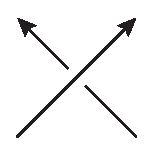
\includegraphics[height=1cm]{crossing+.eps} & 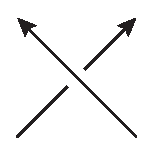
\includegraphics[height=1cm]{crossing-.eps} & 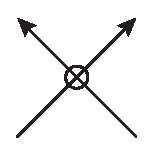
\includegraphics[height=1cm]{v_crossing.eps}\\
\tiny $\sign(c)=+1$ & \tiny $\sign(c)=-1$ & \\
\multicolumn{2}{c}{\small Classical Crossing} & \small Virtual Crossing
\end{tabu}
\qquad
\raisebox{-.5cm}{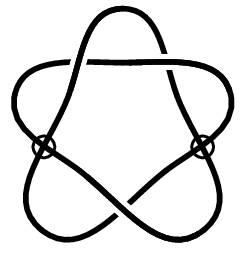
\includegraphics[height=2cm]{virtual_knot}}
\end{frame}


\begin{frame}[fragile]{Virtual Knots}
\begin{defn}
A \myem{virtual knot} is an equivalence class of virtual knot diagrams,
two diagrams being \myem{equivalent(virtually isotopic)} if and only if one can be deformed into the other by planar isotopy and a finite number of applications of generalized Reidemeister moves.
\end{defn}
$$
\raisebox{-.3cm}{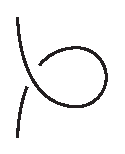
\includegraphics[height=.8cm]{r1-1.eps}} \xleftrightarrow{\mathrm{R1}}
\raisebox{-.3cm}{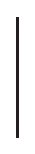
\includegraphics[height=.8cm]{r1-0.eps}}
%\xleftrightarrow{\mathrm{R1}} \raisebox{-.4cm}{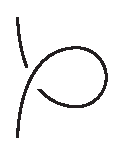
\includegraphics[height=1cm]{r1-2.eps}}
\qquad\quad
\raisebox{-.3cm}{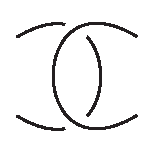
\includegraphics[height=.8cm]{r2-1.eps}} \xleftrightarrow{\mathrm{R2}}
\raisebox{-.3cm}{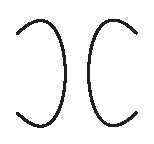
\includegraphics[height=.8cm]{r2-2.eps}}
\qquad\quad
\raisebox{-.3cm}{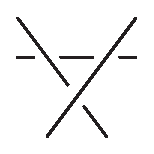
\includegraphics[height=.8cm]{r3-1.eps}} \xleftrightarrow{\mathrm{R3}}
\raisebox{-.3cm}{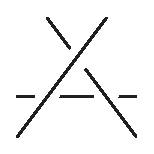
\includegraphics[height=.8cm]{r3-2.eps}}
$$

\hspace*{-.6cm}
$
\raisebox{-.3cm}{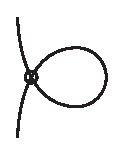
\includegraphics[height=.8cm]{vr1-1.eps}} \xleftrightarrow{\mathrm{VR1}}
\raisebox{-.3cm}{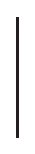
\includegraphics[height=.8cm]{r1-0.eps}}
%\xleftrightarrow{\mathrm{R1}} \raisebox{-.4cm}{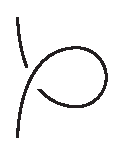
\includegraphics[height=1cm]{r1-2.eps}}
$
\hfill
$
\raisebox{-.3cm}{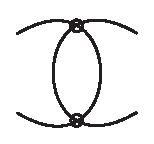
\includegraphics[height=.8cm]{vr2-1.eps}} \xleftrightarrow{\mathrm{VR2}}
\raisebox{-.3cm}{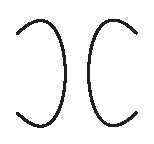
\includegraphics[height=.8cm]{r2-2.eps}}
$
\hfill
$
\raisebox{-.3cm}{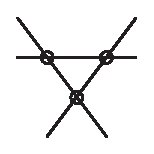
\includegraphics[height=.8cm]{vr3-1.eps}} \xleftrightarrow{\mathrm{VR3}}
\raisebox{-.3cm}{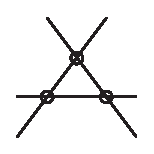
\includegraphics[height=.8cm]{vr3-2.eps}}
$
\hfill
$
\raisebox{-.3cm}{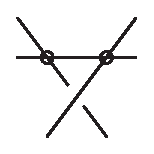
\includegraphics[height=.8cm]{mr3-1.eps}} \xleftrightarrow{\mathrm{VR4}}
\raisebox{-.3cm}{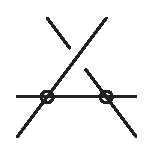
\includegraphics[height=.8cm]{mr3-2.eps}}
$

$$
\raisebox{-.7cm}{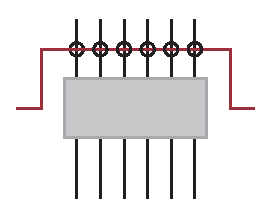
\includegraphics[height=1.6cm]{detour1.eps}} \xleftrightarrow{\mathrm{detour}}
\raisebox{-.7cm}{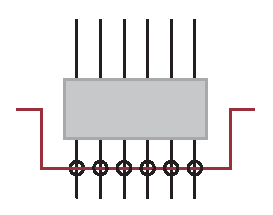
\includegraphics[height=1.6cm]{detour2.eps}}
$$
\end{frame}


\begin{frame}[fragile]{Gauss Diagrams and Gauss Words}
\begin{defn}
A \myem{Gauss diagram $G(D)$} of virtual knot diagram $D$ is a circle
parameterizing the knot with each pair of preimages of crossing of $D$
connected by an {\color{orange}oriented signed chord}.
The chords are oriented from the preimage point on the over strand
to the preimage point on the under strand.
The sign of a chord is the sign of the corresponding crossing.
\end{defn}
$$
\begin{tabu} to .8\linewidth {X[10, c,m] X[c,m] X[10, c,m]}
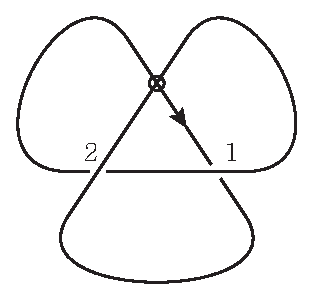
\includegraphics[height=3cm]{trefoil.eps} & &
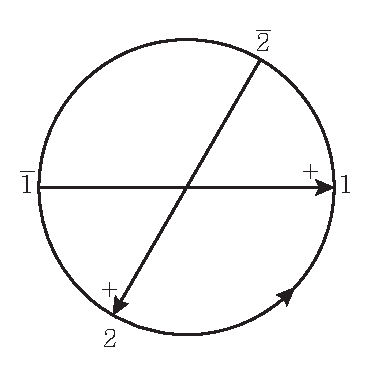
\includegraphics[height=3.4cm]{trefoil_gauss_dia.eps}\\
$1+\overline{2}+\overline{1}+2+$ & &
\end{tabu}
$$
\end{frame}


\begin{frame}[fragile]{Virtual Unknotting Number}
$$
\raisebox{-.4cm}{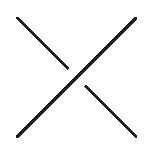
\includegraphics[height=1cm]{1crossing+.eps}}
\xleftrightarrow{\text{Crossing Change}}
\raisebox{-.4cm}{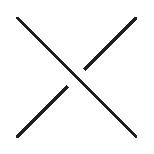
\includegraphics[height=1cm]{1crossing-.eps}}
%\qquad
%\raisebox{-.4cm}{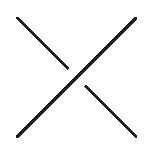
\includegraphics[height=1cm]{1crossing+.eps}}
%\xleftrightarrow{\text{Virtualization}}
%\raisebox{-.4cm}{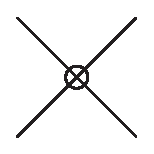
\includegraphics[height=1cm]{1v_crossing.eps}}
$$

\begin{defn}
A \myem{virtual homotopy} between two virtual knot diagrams is a
sequence of virtually isotopies and crossing changes.
\end{defn}

Unfortunately, not every virtual knot is virtually homotopic to the unknot.

\begin{defn}
Suppose $K$ is a virtual knot homotopic to the unknot.
The \myem{virtual unknotting number of K},
denoted by {\color{orange}$\vu(K)$},
is the minimum number of crossing changes
% needed to obtain the unknot from some diagram of the virtual knot $K$.
over all virtual homotopy between $K$ and unknot.
\end{defn}
\end{frame}


\begin{frame}[fragile]{$P$-Invariant}
Let $G(K)$ be a Gauss diagram of a virtual knot $K$.
Then end point of an arrow $a$ of $G(K)$ decompose the circle of $G(K)$ into two open arcs,
$\gamma_1$ and $\gamma_2$.
\begin{itemize}
\item[\myem{$i_i(a)$}:] the set of all arrows($\neq a$) such that their head are on $\gamma_1$
and their tail are on $\gamma_2$
\item[\myem{$i_o(a)$}:] the set of all arrows($\neq a$) such that their head are on $\gamma_2$
and their tail are on $\gamma_1$
\end{itemize}
\[
i(a)=\sum_{c\in i_i(a)}\sign(c)-\sum_{c\in i_o(a)}\sign(c)
\]
$$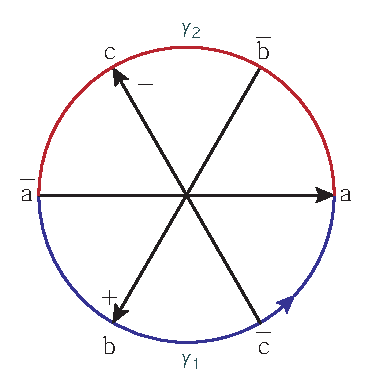
\includegraphics[height=3.5cm]{p-inv.eps}$$
\end{frame}


\begin{frame}[fragile]{$P$-Invariant}
\begin{defn}[A. Henrich]
Define $P(G(K))$ by
\[
P(G(K)) = \sum_{a,\ i(a)\neq 0}\sign(a)t^{|i(a)|}
\]
\end{defn}

\begin{thm}[Byberi and Chernov, 2008]
The polynomial $P(G(K))$ does not depend on a choice of Gauss diagram of the virtual knot $K$.
\[
P(K)=P(G(K))
\]
\end{thm}
\end{frame}

\begin{frame}[fragile]{$P$-Invariant}
\[
\raisebox{-.9cm}{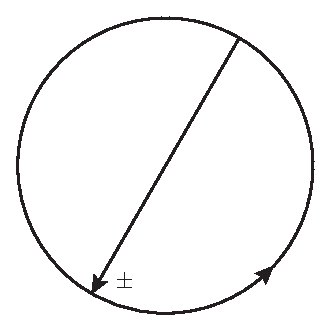
\includegraphics[height=2cm]{flip1.eps}}
\xleftrightarrow{\text{Crossing Change}}
\raisebox{-.9cm}{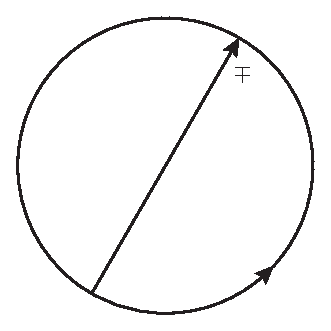
\includegraphics[height=2cm]{flip2.eps}}
\]
\begin{lem}[Byberi and Chernov, 2008]
Let $K$ be a virtually null-homotopic and $P(K)=\sum_{m\in\mathbf{N}}b_mt^m$.
Then
\[
\vu(K)\ge \frac12\sum_{m\in\mathbf{N}}|b_m|
\]
\end{lem}
\vspace{-.3cm}
\begin{proof}
Effects of Crossing change on $\sum|b_m|$ are $\pm2$ or $0$.
\end{proof}
\end{frame}


\begin{frame}[fragile]{Virtual Torus Knot $\vt{p}{q}{n}$}
$$\vt{p}{q}{n} = \raisebox{-2cm}{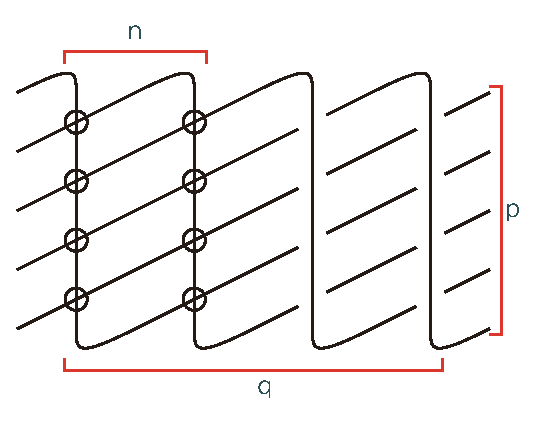
\includegraphics[height=4cm]{vt_pqn.eps}}$$

\begin{lem}[Masuda, 2014]
$\vt{p}{q}{n}$ is virtually homotopic to the unknot.
\end{lem}
\end{frame}


\begin{frame}[fragile]{Lower Bound of $\vu(\vt{p}{q}{n})$}
Let $A$ be the set of all arrow in a gauss diagram of $\vt{q}{q}{n}$.
Define
\begin{align*}
A_0 & = \{a\in A\vert\, i(a)=0\}\\
A_1 & = \{a\in A\vert\, i(a)\neq0\}
\end{align*}

\vspace*{-.3cm}
\begin{thm}[Ishikawa and Yanagi, 2017]
\begin{itemize}
\item $\gcd(p,n)=1$ $\Longrightarrow$ $A_0=\emptyset$
\item $\gcd(p,n)=1$ $\Longrightarrow$ $\displaystyle\vu(\vt{p}{q}{n})\ge\frac{(p-1)(q-n)}{2}$
\item $\displaystyle\vu(\vt{p}{q}{n})\ge\frac{(p-1)(q-n)-|A_0|}{2}$
\end{itemize}
\end{thm}
\vspace*{-.3cm}
\begin{proof}
All crossing of $\vt{p}{q}{n}$ are positive.
Thus
\[
\sum_{m\in\mathbf{N}}|b_m| = |A_1| = |A| - |A_0| = (p-1)(q-n) - |A_0|
\]
\end{proof}
\end{frame}


\section{Main Result}

\begin{frame}[fragile]{Main Result}
\[
\vu(\vt{p}{q}{q-1}) = \frac{p-1}{2} - \frac{\gcd(p,q-1)-1}{2}
\]
\medskip

\myem{Lower Bound:} Modify Ishikawa and Yanagi's $P$-invariant arguments

\myem{Upper Bound:} Find a virtual null-homotoy and count the number of crossing changes

\end{frame}


\section{Lower Bound of $\vu(\vt{p}{q}{q-1})$}

\begin{frame}[fragile]{Gauss Word of $\vt{p}{q}{q-1}$}
\centerline{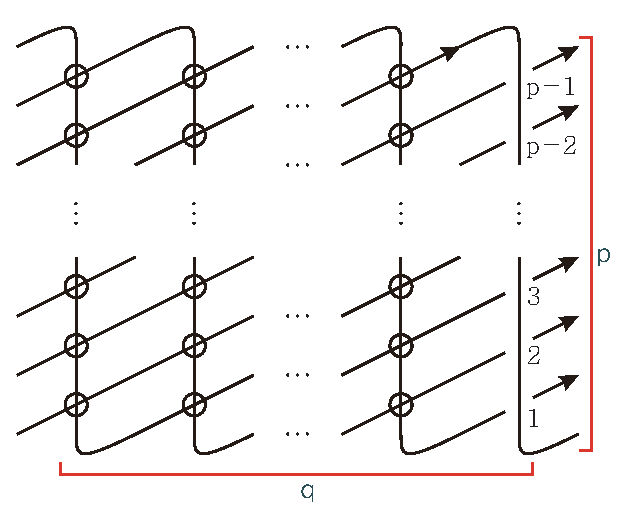
\includegraphics[height=4cm]{gauss_vt.eps}}
\[
\overline{p-1}+\overline{p-2}+\cdots+\overline{2}+\overline{1}+\prod_{i=1}^{p-1}\left[(qi\mod p)+\right]
\]
\end{frame}


\begin{frame}[fragile]{Another Formula of $i(a)$}
Let $a$ be an arrow in the gauss diagram of $\vt{p}{q}{q-1}$.
Define
\begin{itemize}
\item[\myem{$I(a)$}:] the set of all arrows($\neq a$) such that their head are on $\gamma_1$
\item[\myem{$O(a)$}:] the set of all arrows($\neq a$) such that their tail are on $\gamma_1$
\end{itemize}

\begin{lem}
Let $D$ be a gauss diagram of a virtual knot whose crossings are all positive.
Then for any arrow $a$ in $D$,
\[
i(a) = |I(a)| - |O(a)|
\]
\end{lem}
\vspace{-.5cm}
\begin{proof}
\vspace{-.3cm}
\begin{align*}
i(a) & = i_i(a) - i_o(a)\\
& = |I(a) - I(a)\cap O(a)| - |O(a) - O(a)\cap I(a)|\\
& = |I(a)| - |O(a)|
\end{align*}
\end{proof}
\end{frame}


\begin{frame}[fragile]{$A_0$ of $\vt{p}{q}{q-1}$}
\begin{thm}
Let $A$ be the set of all arrows of a gauss diagram of $\vt{p}{q}{q-1}$,
and $A_0=\{c\in A\vert\, i(c)=0\}$.
Then
\[
|A_0|= \gcd(p,q-1)-1.
\]
\end{thm}

\hfill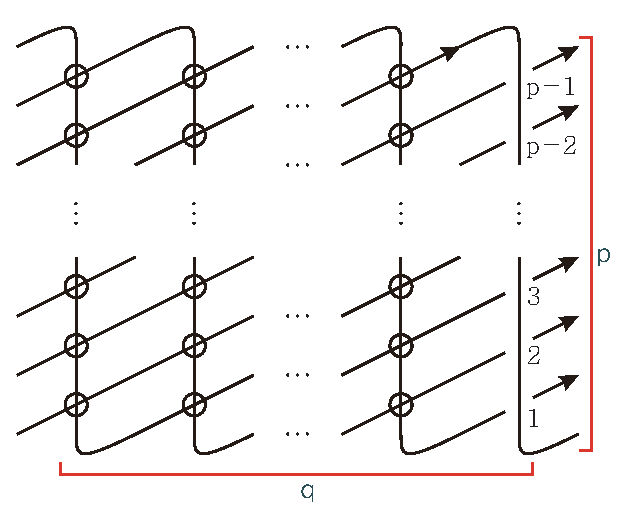
\includegraphics[height=4cm]{gauss_vt.eps}\hfill
\vspace{-.3cm}
\[
\overline{p-1}+\overline{p-2}+\cdots+\overline{2}+\overline{1}+\prod_{i=1}^{p-1}\left[(qi\mod p)+\right]
\]
\end{frame}


\begin{frame}[fragile]{Proof of Theorem}
Suppose that $\overline{k}+$ and $k+$($1\le k\le p-1$) are corresponding to the arrow $a$
in the gauss word of $\vt{p}{q}{q-1}$.

Let $r$ be the smallest natural number such that \myem{$rq\equiv k\mod p$}.
Then
\begin{align*}
O(a) & = \{\overline{1}+,\overline{2}+,\ldots,\overline{k-1}+\}\\
I(a) & = \{(q\mod p)+, (2q \mod p)+,\ldots,((r-1)q\mod p)+\}
\end{align*}
Thus $i(a)=0$ $\Leftrightarrow$ $|O(a)|=|I(a)|$ $\Leftrightarrow$ $r=k$.

Since $1\le k\le p-1$,
\begin{align*}
r = k & \Leftrightarrow kq \equiv k \mod p\\
& \Leftrightarrow k(q-1)\equiv 0 \mod p\\
& \Leftrightarrow k = \frac{np}{q-1}\ \text{for some $n\in\mathbf{N}$}
\end{align*}
\end{frame}


\begin{frame}[fragile]{Proof of Theorem}
Let $a=\gcd(p,q-1)$, then
\begin{align*}
r = k & \Leftrightarrow k=\frac{np/a}{(q-1)/a}\ \text{for some $n\in\mathbf{N}$}
\end{align*}
Since $p/a$ and $(q-1)/a$ are relative prime, in order for k to be a natural number,
\[
n = \frac{\alpha(q-1)}{a}
\]
for some natural number $\alpha$.
Thus
\begin{align*}
r = k & \Leftrightarrow k=\frac{\alpha p}{a}
\end{align*}
Since $1\le k\le p-1$, $1\le\alpha\le a-1$.

Because $k$ is uniquely determined by $\alpha$,
\[
|A_0| = a-1 = \gcd(p,q-1) - 1\tag*{$\square$}
\]
\end{frame}


\begin{frame}[fragile]{Lower Bound of $\vu(\vt{p}{q}{q-1})$}
\begin{thm}
\[
\vu(\vt{p}{q}{q-1}) \ge \frac{p-1}{2} - \frac{\gcd(p,q-1)-1}{2}
\]
\end{thm}
\begin{proof}
\begin{align*}
\vu(\vt{p}{q}{q-1}) & \ge \frac{1}{2}\sum|b_m|\\
& = \frac{1}{2}\left(|A| - |A_0|\right)\\
& = \frac12\left\{(p-1) - [\gcd(p,q-1)-1]\right\}
\end{align*}
\end{proof}
\end{frame}



\section{Upper Bound of $\vu(\vt{p}{q}{q-1})$}

\begin{frame}[fragile]{Some Virtual Homotoy}
\begin{align*}
\raisebox{-.9cm}{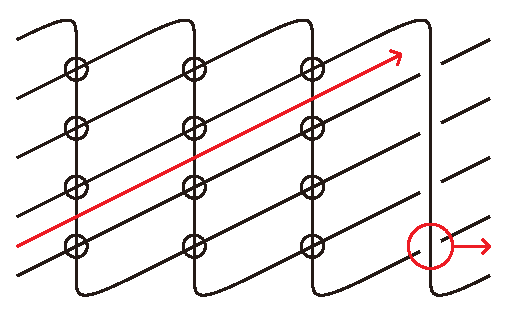
\includegraphics[height=2cm]{new_op1-1.eps}}
& \xlongrightarrow{\text{VR4s}}
\raisebox{-.9cm}{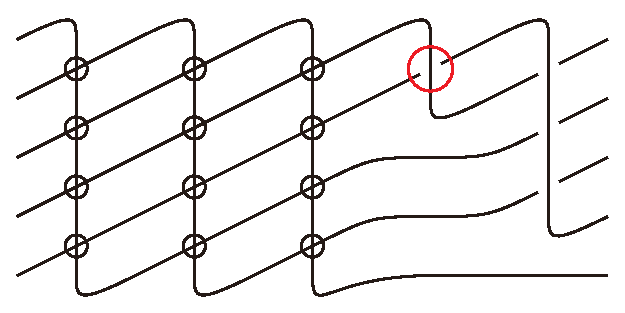
\includegraphics[height=2cm]{new_op1-2.eps}}\\
& \xlongrightarrow{\text{Crossing Change}}
\raisebox{-.9cm}{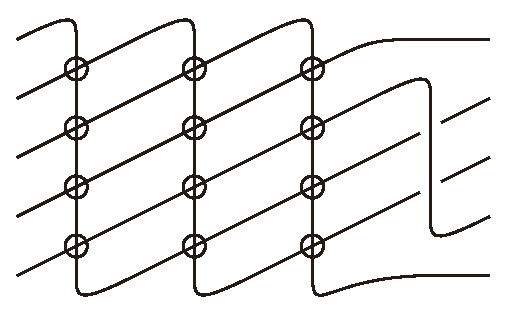
\includegraphics[height=2cm]{new_op1-3.eps}}
\end{align*}
\end{frame}


\begin{frame}[fragile]{Some Virtual Homotoy}
\begin{align*}
& \raisebox{-.9cm}{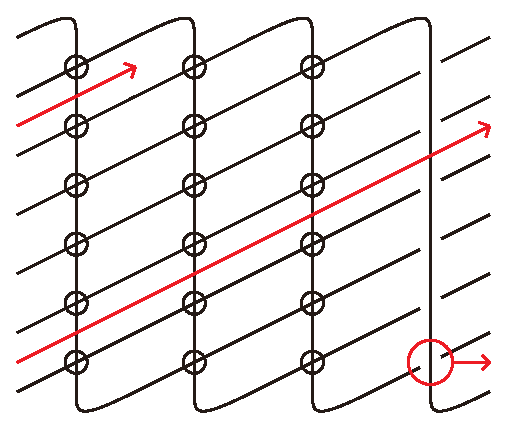
\includegraphics[height=1.8cm]{new_op2-1.eps}}
\xlongrightarrow{\text{VR4s}}
\raisebox{-.9cm}{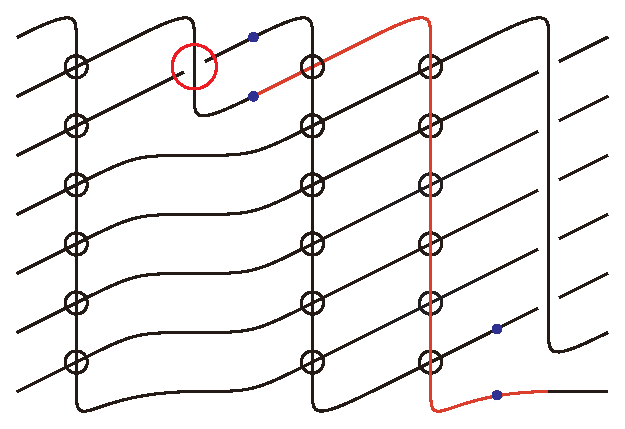
\includegraphics[height=1.8cm]{new_op2-2.eps}}
\xlongrightarrow{\text{Detour}}
\raisebox{-.9cm}{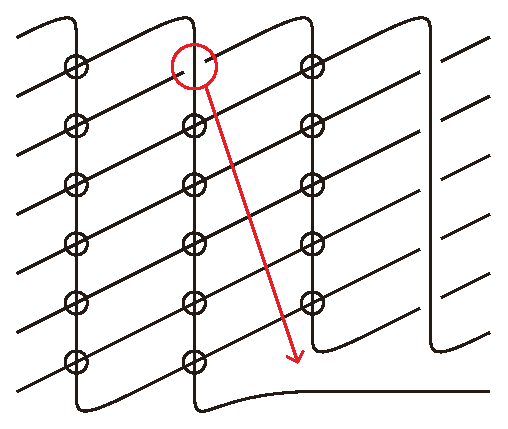
\includegraphics[height=1.8cm]{new_op2-3.eps}}
\xlongrightarrow{\text{VR4s}}\\
& \raisebox{-.9cm}{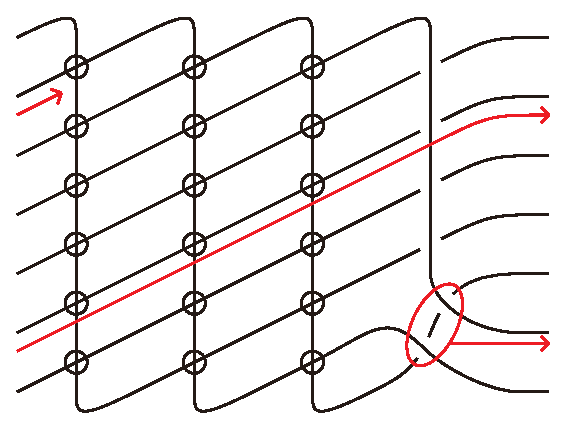
\includegraphics[height=1.8cm]{new_op2-4.eps}}
\xlongrightarrow{\text{VR4s}}
\raisebox{-.9cm}{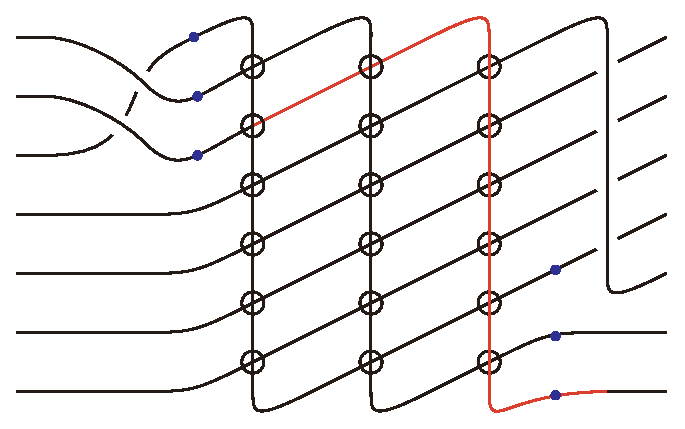
\includegraphics[height=1.8cm]{new_op2-5.eps}}
\xlongrightarrow{\text{Detours}}
\raisebox{-.9cm}{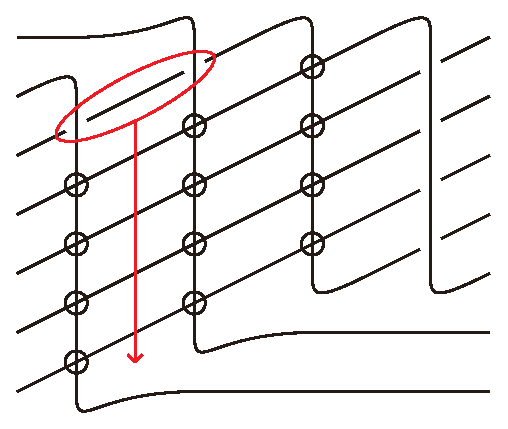
\includegraphics[height=1.8cm]{new_op2-6.eps}}
\xlongrightarrow{\text{Detour}}\\
& \raisebox{-.9cm}{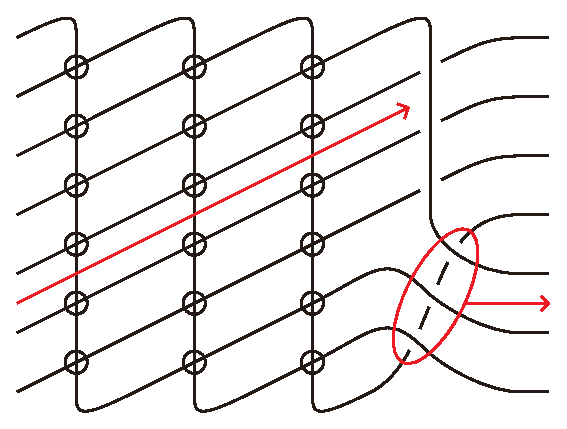
\includegraphics[height=1.8cm]{new_op2-7.eps}}
\xlongrightarrow{\text{VR4s}}
\raisebox{-.9cm}{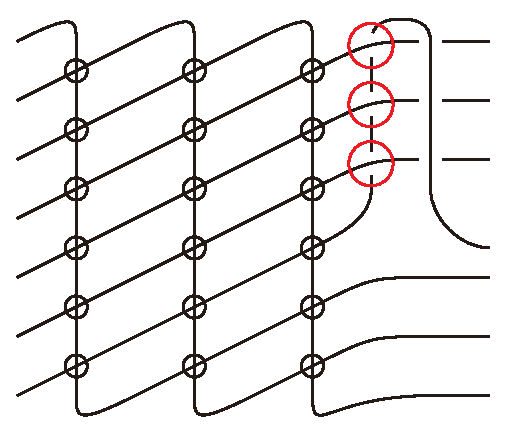
\includegraphics[height=1.8cm]{new_op2-8.eps}}
\xlongrightarrow{\text{Crossing Change}}
\raisebox{-.9cm}{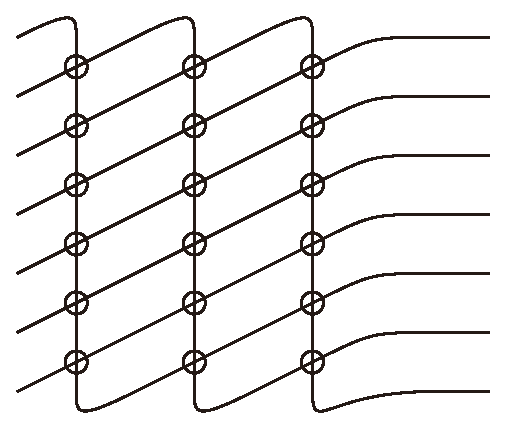
\includegraphics[height=1.8cm]{new_op2-9.eps}}
\end{align*}
\end{frame}


\begin{frame}[fragile]{$M$-Gauss Word}
\begin{defn}
A Gauss word
\[
\overline{r}+\overline{r-1}+\cdots\overline{2}+\overline{1}+a_1+a_2+\cdots+a_r+
\]
is called \myem{$M$-Gauss word} if
\begin{itemize}
\item $a_i+a_{r-i+1}=r$ for all $1\le i\le r$
\item if $a_k=1$, then $a_{k+i}=a_i+1$ for all $1\le i\le r-k$ 
\end{itemize}
Especially, if $a_1=1$, then it is called \myem{$M1$-Gauss word}.
\end{defn}
\end{frame}


\begin{frame}[fragile]{$RVT_{p,q}^m$}
\[
RVT_{p,q}^m =\quad \raisebox{-2.4cm}{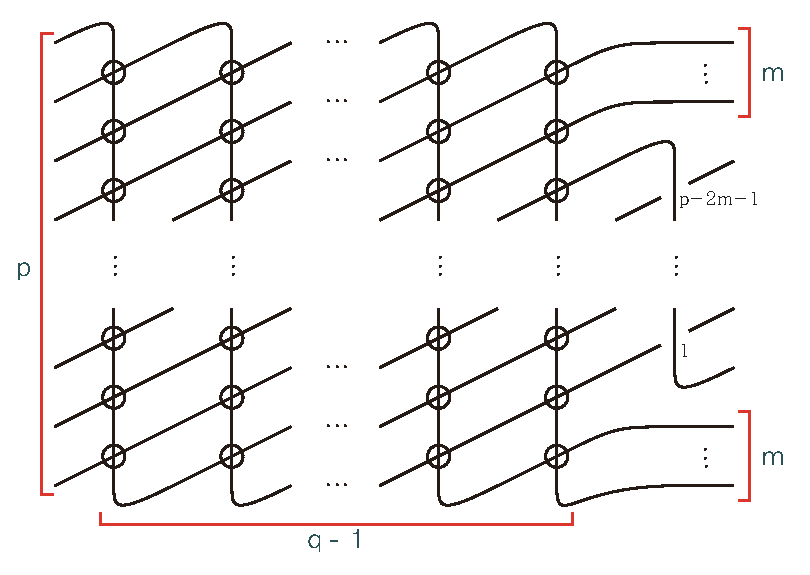
\includegraphics[height=5cm]{rvt.eps}}
\]
\begin{thm}
The Gauss word of a gauss diagram of $RVT_{p,q}^m$ is $M$-Gauss word.
\end{thm}
\end{frame}


\begin{frame}[fragile]{$L$-Move}
\myem{$L$-Move: $L(a,b,c)$}
\[
\raisebox{-.6cm}{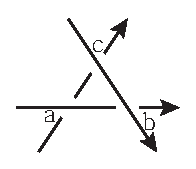
\includegraphics[height=1.5cm]{l1.eps}}
\xrightarrow{\text{R3}}
\raisebox{-.6cm}{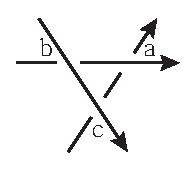
\includegraphics[height=1.5cm]{l2.eps}}
\xrightarrow{\text{Relabeling}}
\raisebox{-.6cm}{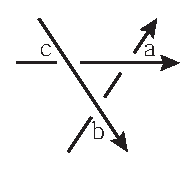
\includegraphics[height=1.5cm]{l3.eps}}
\]
\[
\raisebox{-1.4cm}{\includegraphics[height=3cm]{gl1.eps}}
\xrightarrow{\text{R3}}
\raisebox{-1.4cm}{\includegraphics[height=3cm]{gl2.eps}}
\xrightarrow{\text{Relabeling}}
\raisebox{-1.4cm}{\includegraphics[height=3cm]{gl3.eps}}
\]
\end{frame}


\begin{frame}[fragile]{$P$-Move}
\myem{$P$-Move: $P(a,b)$}
\[
\raisebox{-.6cm}{\includegraphics[height=1.5cm]{p1.eps}}
\xrightarrow{\text{Crossing Change}}
\raisebox{-.6cm}{\includegraphics[height=1.5cm]{p2.eps}}
\xrightarrow{\text{R3}}
\raisebox{-.6cm}{\includegraphics[height=1.5cm]{p3.eps}}
\]
\end{frame}


\begin{frame}[fragile]{$H$-Move}
\myem{$H$-move} on $M$-Gauss word
\[
\overline{r}+\overline{r-1}+\cdots+\overline{1}+a_1+a_2+\cdots+a_r+
\]
is defined by
\begin{align*}
& \overline{r-2x}+\overline{r-2x-1}+\cdots\overline{2}+\overline{1}+\\
&\quad\prod_{i=1}^{r-kx}[a_i+]\prod_{i=r-kx+2}^{k-1}[(a_i-1)+]\prod_{i=1}^{r-kx}[(a_i-1)+]\prod_{i=r-kx+2}^{k-1}[(a_i-2)+]\\
&\cdots\prod_{i=r-kx+2}^{k-1}[(a_i-x)+]\prod_{i=1}^{r-kx}[(a_i-x)+],
\end{align*}
where $a_k=1$ and $x=\left[\frac{r}{k}\right]$
\begin{thm}
$H$-move is a sequence of $L$-moves and $P$-moves.
Moreover, the number of the removed crossing by applying an $H$-move is twice time of the number of crossing change in the $H$-move.
\end{thm}
\end{frame}


\begin{frame}[fragile]{Virtual Homotopy of $\vt{p}{q}{q-1}$}
\begin{thm}
By applying an $H$-move, $RVT_{p,q}^m$ can be deformed to $RVT_{p,q}^{m+x}$, where $x=\left[\frac{p-2m-1}{k}\right]$.
\end{thm}

\begin{cor}
By applying finite number of $H$-moves, $\vt{p}{q}{q-1}$ can be deformed unknot.
\end{cor}

\[
\vt{p}{q}{q-1}=RVT_{p,q}^0\xrightarrow{\text{$H$-move}}RVT_{p,q}^{m}\xrightarrow{\text{$H$-move}}RVT_{p,q}^{m+x}\xrightarrow{\text{$H$-move}}\cdots\xrightarrow{\text{$H$-move}}\text{Unknot}
\]
\end{frame}


\begin{frame}[fragile]{Upper Bound of $\vt{p}{q}{q-1}$}
\begin{lem}
After applying any $H$-move, the number of crossing such that $i(c)=0$ does not change.
Moreover, the crossing with $i(c)\neq0$ can be removed by applying an $H$-move.
\end{lem}

\begin{thm}
\[
\vu(\vt{p}{q}{q-1}) \le \frac{p-1}{2} - \frac{\gcd(p,q-1)-1}{2}
\]
\end{thm}
\end{frame}


\begin{frame}[fragile]{Proof of Theorem}
%Let $d$ be the number of crossing after virtual homotopy of $\vt{p}{q}{p-1}$.
%Then $p-1-d$ crossings are removed.
%Hence the number of crossing change in this virtual homotoy is $\frac{p-1-d}{2}$.
%
Since $|A_1|=(p-1)-[\gcd(p,q-1)-1]$,

after $\frac{p-1}{2} - \frac{\gcd(p,q-1)-1}{2}$ times crossing change,

resulting virtual knot is $RVT_{p,q}^{m}$, where $m=\frac{p-1}{2} - \frac{\gcd(p,q-1)-1}{2}$.


Moreover, the Gauss word of the $RVT_{p,q}^{m}$ is
\[
\overline{d}+\overline{d-1}+\cdots\overline{2}+\overline{1}+1+2+\cdots(d-1)+d+,
\]
where $d=\gcd(p,q-1)-1$.

It is a Gauss word of the torus knot $T(d+1,1)(\cong\text{unknot})$.

Therefore
\[
\vu(\vt{p}{q}{q-1}) \le \frac{p-1}{2} - \frac{\gcd(p,q-1)-1}{2}
\]
\end{frame}


\begin{frame}[fragile]{}
\myem{\huge Thank you for listening.}
\end{frame}
\end{document}





